\chapter{Separating Polygonal Sets with Minimum Sets of Lines}
\thispagestyle{myheadings}

After two chapters' discussion on covering perimeters or regions, which is essentially separating 
some critical polygonal regions from the outside workspace. 
This chapter digs deeper into this problem by studying the separation of more than two regions. 
To simplify the problem, a line-of-sight sensing model will be adopted, where each sensor can cover
an unobstructed line segment like a laser beam. Also, the regions are assumed to be polygonal.

The objective in this case is to minimize the number of sensors used to separate these polygonal sets 
at the existence of obstacles.
% The main objective here is to minimize the number of sensor used.
The problem is NP-hard even for the problem of separating two sets of regions with the minimum number of lines. 
Still, integer programming can provide a near-optimal solution for around 20 objects in a reasonable amount of time. 

\section{Introduction}
Consider the scenario where one or more rogue agents (e.g., criminals) may be hiding in several isolated regions in a 2D workspace. To prevent them from potentially escaping from these regions to other nearby vulnerable regions, we may wish to set up line-of-sight sensors to detect if rogue agents attempt to escape. For the setup, a natural question one may ask is: what is the minimum number of line segments that are needed to form the desired barrier? The same setting finds many other practical applications, for example, for the identical setting, we may use the deployed sensors to track the movement of agents between different set of regions, e.g., understanding the flow of people between residential areas to commercial areas, which can benefit large-scale decision making, e.g., to help properly allocating resources for improving the city infrastructure. 
%
Alternatively, the computed line segments can serve as patrolling routes for autonomous agents (robots or humans) for actively monitoring intrusions, where the agents can always keep tracking events along the segments for which they are responsible.

%Barrier forming \cite{}, i.e. separating multiple sets of objects from each other,
%where each set may contain multiple scattered objects mix among other object sets, finds many real-world applications,
%e.g., erecting security fences around buildings,
%isolating different groups of agents (e.g., people, animals), 
%designing routes for patrolling robots to detect invaders, and so on. 
%multi-agent search for rouge agents, and so on. 
%These applications shares the common objective of better coverage or sensing of the environment with guards. 
%In reality, the types of barriers varies from barriers with range sensibility like lidar, visibility-based barriers like cameras or guards, to physical straight line fences or walls.
%
Motivated by the above stated scenarios and inspired by earlier research in robotics on barrier forming \cite{kloder2007barrier,kloder2008partial}, i.e., erecting barriers for separating regions of interest, in this chapter, we examine the variation of finding the minimum number of straight line segments for isolating multiple sets of points of polygons in a two-dimensional workspace. 
Fig~\ref{fig:bf-ex}[left] illustrates an instance where three colored polygonal sets are to be separated from each other and the grey polygons are obstacles. Fig~\ref{fig:surf-ex}[right] shows a possible solution which is fairly non-trivial 
to obtain. 
%
%The problem finds applications in many practical scenarios where geometric separation is needed, for example, the deployment of a minimum set of  line-of-sight security beams to guard critical areas from intrusions. 
%dividing different rooms in a floor or buildings from each other to prevent the %spread of virus or contagious diseases,
%designing the surveillance routes for guards that walk on a straight route,
%building fences for regions among different security level that are not allowed 
%to have connections, and so on. 

\begin{figure}[t]
    \centering
    \includegraphics[width=\columnwidth]{chapters/bf/fig/intro_pic.png}
    \caption[Example of barrier forming for separating three sets of complex polygonal shapes]
    {Example of barrier forming for separating three sets of complex polygonal shapes. Different colors represent different sets with the grey ones representing obstacles. The red line segments are the barriers computed by our algorithm.}
    \label{fig:bf-ex}
    \vspace{-0.2in}
\end{figure}
As a summary of this work and its contributions, we study three settings in using line segments to separate sets of disjoint geometric shapes in a 2D workspace: (1) separating point sets, (2) separating point sets among polygonal obstacles, and (3) separating polygonal sets among polygonal obstacles. 
%
Whereas all three settings are NP-hard to optimally solve, we derive an effective method for computing optimal solutions for the first two settings, capable of handling tens of objects (points and/or polygons) partitioned into multiple sets. 
%
The  method first systematically computes candidate barrier set containing a minimum separating barrier, and then builds a novel integer programming model for finding the minimum barrier. 
%
Following a similar approach, we also develop a method that computes solutions for the third setting that is proven to be at least $2$-optimal. 
%
We provide theoretical analysis that shed some light on why the setting involving polygonal sets is more difficult to solve.
%
Extensive simulation study corroborates the effectiveness of our algorithms. 

%Our contribution to barrier forming is, in summary, formulating the problem of minimizing
%the line segment barriers used with respect to different kinds of object sets (point object and polygonal object). 
%For barrier forming among sets of point objects, we provide effective integer programming based method to obtain the optimal solution.
%For the general polygonal objects, our method can provide a guaranteed 2-OPT solution.
%We also perform evaluations on four different settings to show
%the effectiveness of the proposed method.


\noindent\textbf{Related Work}.
Our investigation of barrier forming has its origins from several research areas.
In the study of pursuit evasion or more generally differential games \cite{ho1965differential,isaacs1999differential,hajek2008pursuit,tovar2009sensor,simov2000pursuit,guibas1997visibility,kameda2006online,kirousis1986searching, sachs2004visibility,lau2005optimal, yu2011shadow, olsen2022robust}, 
% flash light searcher, 1-2 inf searcher
such scenarios often happen where several agents are tasked to search an environment for hidden rogue agents or to protect critical regions from outsider invaders, which amount to creating and maintaining static or dynamic barriers of some form.  
%
Among the approaches taken in finding solutions for these problems, some resort to discretize the environment into graph representations and conduct search over them \cite{kirousis1986searching, sachs2004visibility}, while others adopt probabilistic reasoning \cite{lau2005optimal, yu2011shadow}. 
%
In particular, Tovar et al. \cite{tovar2009sensor} studied a problem that examines how to untangle sensor beam crossings to reason about the state of a robot, and use the insight to build algorithms for driving a robot to a desired state. In a sense, their study can be viewed as studying a problem that is a dual of the problem that we study here. 

%\textcolor{red}{JJ's edit location}

Barrier forming problems can also be seen as a type of sensor coverage problem. 
%
A series of study of perimeter defense/guarding problems aim at covering the boundaries of some regions to protect them from the outside \cite{shishika2020cooperative, macharet2020adaptive, fenghangaoyu2019efficient, fengyu2020optimally}, which share similar motivations. 
The barrier forming problem has more flexible solutions by not fixing the specific boundaries to secure for the critical regions,
which can be more general and closer to reality.
In \cite{kloder2007barrier}, the authors solved the barrier coverage problem optimally under non-trivial environment to minimize the total length of the barriers between two groups of polygonal objects. 
To tackle the proposed problem, a novel and efficient network-flow based method is applied. 
In \cite{abrahamsen2020geometric}, the work is extended to multiple groups of objects.
The following work \cite{kloder2008thesis} includes a similar problem formation to the problem studied in this chapter, where the objective is minimizing the number of fixed-length line segments used. 
%
However, that proposed method in \cite{kloder2008thesis} uses Tarski sentence \cite{tarski1949decision} which, to our knowledge, does not have very effective method to duel with.

This work is closely related to several problems in computational geometry, especially point set shattering which seeks a complete separation among a single set of points \cite{freimer1991complexity, har2020separating}. 
Bichromatic point sets or polyherdral separation problem uses wedges, axis-aligned lines, chords, parallel lines, or circles to separate two sets of points or polyhedra \cite{devillers2001separating,armaselu2017geometric,boissonnat2001circular, demaine2005separating}. 
Work on these problems often put on specific constraints such as working with convex objects or simple polygons without holes, adopting non-crossing or parallel lines as the separator, and so on. 

\noindent \textbf{Chapter Structure}.
The rest of the chapter starts with formulating the barrier formation problem and 
introducing the three variants studied in ~\ref{sec:bf-preliminary}. 
Then, we describe the structure analysis of the problem in ~\ref{sec:bf-structure}, which will base the algorithm
proposed in ~\ref{sec:bf-algorithm}. Lastly, in ~\ref{sec:bf-evaluation} we evaluate the algorithm on four different scenarios. %\r{associate each with a specific section.}

%  methods take
% The problem of constructing a set of barriers appears in various robotics applications 


% Barrier forming is studied in various domains.
% In the pursuit evasion game, barriers were constructed to perform 
% area scan, moving target persuasion \cite{yu2011shadow, tovar2009sensor} etc.
% In computational geometry,
% barrier forming has relevance to several problem: 
% Regarding separating polygons, 
% the study of barrier coverage problem introduces a network flow-based algorithm 
% for computing the minimum total distance separation for two sets of polygons 
% with the existence of obstacles\cite{kloder2007barrier, kloder2008thesis}.
% In \cite{kloder2008thesis}, the author explored barrier forming with minimum number of 
% fixed-length line segments, while it is still important to find high performance
% solution for such problem.\label{sec:bf-intro}

\section{Preliminaries}\label{sec:bf-preliminary}
In boundary defense with heterogeneous defenders (\prob), there are $k$ defenders (which may be robots and/or other types of agents) with speeds $v_1,\dots,v_k$, where each defender is modeled as a point in some domain $\mathcal E = \mathbb R^2$ or $\mathbb R^3$.
The defenders live on a lower dimensional subspace of $\mathcal E$ (i.e., some boundary of a subset of $\mathcal E$).  
There are also $n$ attack events $\big\langle loc_i, t_i\big\rangle_{i=1}^{n}$, where each attack event is a pair $\big\langle loc, t\big\rangle$ in which $loc$ is the
location of the attack and $t$ is the time it happens. 
The $i^{{th}}$ attack is intercepted by a defender only if the defender is located at $loc_i$ at time $t_i$.
For initialization, we denote the initial locations of the $k$ defenders at $t=0$ as $loc^{1},\dots, loc^{k}$. 

Following the definition in \cite{adler2022role}, we define the horizon of the defenders as follows,
\begin{definition}[Horizon]
The (look ahead) \textit{horizon} $T$ of the defenders is defined as the amount of time defenders can peek into the attack sequence in the future. That is, given the current time $t$, and a horizon $T$, defenders have access to complete information on attacks happening on or before $t+T$. 
\end{definition}

Now, we provide formulations of the two versions of the \prob problem studied in this paper. In the infinite horizon setting, $T = \infty$, all attack events are given in a single batch.

\begin{problem}[Infinite-horizon \prob]\label{prob:1}
Given $k$ defenders with speed $v_1, \dots, v_k$ and initial locations $loc^1, \ldots, loc^k$, and $n$ attack events $\big\langle loc_i, t_i\big\rangle_{i=1}^{n}$, intercept as many attacks as possible. 
\end{problem}

In a finite-horizon setting, the attack events are not all revealed at $t=0$ but are given as a stream of attacks $\big\langle loc_i, t_i\big\rangle_{i=1}^{\infty}$. The defenders can only know the attack events within a horizon or time window of $T < \infty$ in the future.

\begin{problem}[Finite-horizon \prob]\label{prob:2}
There are $k$ defenders with speed $v_1, \dots, v_k$ and initial locations $loc^1, \ldots, loc^k$, and a stream of attack events.
%
At each time instance $t$, the defenders only know attack events happening no later than time $T$ in the future (i.e. $t_i \le t+T$).
%
Intercept as many attacks as possible. 
\end{problem}

We introduce here two useful notations: $next(a, d)\ (a\in[0, n],\ d\in[1,k])$ and $prev(a, d)\ (a\in[1,n],\ d \in [1,k])$.
They are defined as
\begin{align}
next(a, d) = \{ a'| dist(loc_a, loc_{a'}) \leq v_d \cdot (t_{a'} - t_a) \}    \\
prev(a, d) = \{ a'| dist(loc_a, loc_{a'}) \leq v_d \cdot (t_a - t_{a'}) \}    
\end{align}
where $dist(x,y)$ denotes the distance between location $x$ and $y$. 
In other words, $next(a, d)$ is the set of 
attack events that can be reached from the location of the $a^{th}$ attack event by defender $d$. 
And $prev(a,d)$ is the set of attack events from whose location defender $d$ can reach the $a^{th}$ attack event. 
Additionally, $next(0, d)$ denotes the set of attack events that can be reached by defender $d$ from its initial location.
Similarly, $prev(a, d)$ contains $0$ if defender $d$ can reach the location of attack $a$ from its initial location.
Fig.~\ref{fig:next_prev} gives an example for defender $1$.

\begin{figure}[h]
    \centering
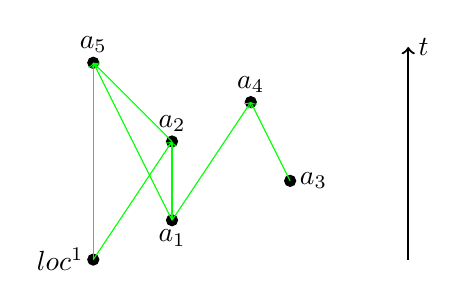
\begin{tikzpicture}
%\draw[black, thick, ->] (0,0) -- (4.5,0) node[anchor=south]{location};
\draw[black, thick, ->] (5,0) -- (5, 2.7) node[anchor=west]{$t$};

\filldraw[black] (1, 0) circle (2pt) node[anchor=east](iloc1){$loc^1$};

\filldraw[black] (2,0.5) circle (2pt) node[anchor=north](a1){$a_1$};
\filldraw[black] (2,1.5) circle (2pt) node[anchor=south](a2){$a_2$};
\filldraw[black] (3.5,1) circle (2pt) node[anchor=west](a3){$a_3$};
\filldraw[black] (3,2) circle (2pt) node[anchor=south](a4){$a_4$};
\filldraw[black] (1,2.5) circle (2pt) node[anchor=south](a5){$a_5$};

\draw[green, thin, ->] (iloc1.east) -- (a2.south);
\draw[green, thin, ->] (iloc1.east) -- (a5.south);

\draw[green, thin, ->] (a1.north) -- (a2.south);
\draw[green, thin, ->] (a1.north) -- (a4.south);
\draw[green, thin, ->] (a1.north) -- (a5.south);
\draw[green, thin, ->] (a2.south) -- (a5.south);
\draw[green, thin, ->] (a3.west) -- (a4.south);

\end{tikzpicture}
    \caption{Illustration of an example of reachability between different attack events for defender $1$.  
    For example, $next(1, 1) = \{2,4,5\}$, $next(0,1)=\{2,5\}$, $prev(2, 1) =\{0, 1\}$, $prev(1,1)=\varnothing$.
    $loc^1$ cannot reach $a_1$ since $v_1$ is not sufficiently large. For the same reason, defender $1$ cannot reach $a_3$ from $a_1$.
    }
    \label{fig:next_prev}
\end{figure}



\section{Structural Analysis}\label{sec:bf-structure}

\section{Structural Analysis}
Given that barrier forming problems studied in this work are NP-hard, a natural algorithmic choice for addressing the challenge is through exploring  mathematical programming.
%
To that end, a model must be built that selects from candidate barriers, which in turn requires the construction of a representative set of barrier candidates, a rather non-trivial task. 
%
The set of candidate barriers should satisfy two conflicting constraints: (1) it should contain a minimum set line segments that achieves the desired separation and (2) its size should not be too big that it will cripple the barrier selection process. 
%
Through careful structural analysis, we notice that the barriers to be considered can be limited to \emph{tangent} or \emph{bitangent} line segments. A tangent line segment, with respect to an object or an obstacle, is a line that passes through a vertex or an edge of the object/obstacle but does not intersect its interior. A bitangent is a line segment that is tangent to two objects and/or obstacles. 
%
This allows us to significantly reduce the number of candidates to be examined at the later selection stage.

\begin{theorem}\label{theorem:sin_tan}
For any $k$ sets of polygonal or point objects $S_1, \dots, S_k$ in the workspace $\mathcal W$, the set of line segments that are tangential to the objects and obstacles contains a set of minimum cardinality that separates $S_1, \dots, S_k$. 
\end{theorem}


\begin{proof}

% We prove that there exists a set of lines with minimum cardinality that separates $S_1, \dots, S_k$, and consists of only lines tangent to object vertices. 
Consider a set of line segments $L^*$ with minimum cardinality that separates $S_1,\dots, S_k$. 
Without loss of generality, we assume all line segments in $L^*$ do not end in the free space, i.e., each line segment in $L^*$ ends
at either object boundaries or workspace boundaries.
If some line segment in a minimum barrier is not tangent to any object vertex, denoted it as $\ell=OA$ (shown in ~\ref{fig:proof}), we show that it can be replaced by a line segment that is tangent to some object vertex. 
%
Fix one end of $\ell$, $O$ in this case, and rotate $\ell$ around $O$ in both clockwise and counterclockwise directions until it hits some object vertex and becomes tangential to the object.
%
Denote the two line segments resulting from clockwise rotation and counterclockwise rotation as $\ell_1'=OB$ and $\ell'_2=OC$, respectively. 

We show $\ell$ can be replaced with $\ell_1'$ or $\ell_2'$. 
If this is not the case,
since replacing $\ell$ with $\ell_1'$ cannot make the separation work, there must be some point $P_1$ between $AB$ that is path connected to some point in the other class without crossing any line segments in $L^*$ when $\ell$ is replaced with $\ell'_1$. Denote the point as $D_1$ and the path as $path_1$. 
The same analysis goes for $\ell'_2$, that if $\ell$ cannot be replaced by $\ell_2$ then there is some point $P_2$ in $AC$ and path $path_2$ that connects $P_2$ to some other point $D_2$ in a different class and crosses segment $\ell$ but not $\ell_2'$. 
Since there are no objects or obstacles inside triangle $OCB$, we can assume the parts of $path_1$ and $path_2$ inside triangle $OCB$ are straight lines.
So, $path_1$ and $path_2$ must cross each other at some point. 
Denote the cross point as $Q\in path_1 \cap path_2$. 
Then, $path_1 = path_{11} (from\ P_1\ to\ Q) + path_{12} (from\ Q\ to\ D_1)$ and $path_2 = path_{12} (from\ P_2\ to\ Q) + path_{22} (from\ Q\ to\ D_2)$. 
Path $p_{11} + p_{22}$ connects $P_1$ to $D_2$, and $p_{21} + p_{12}$ connects $P_2$ to $D_1$, one of which must not cross $\ell$. 
This leads to a contradiction to the fact that the original line set $L^*$ separates the $k$ classes of objects.

Therefore, each non-tangent line segment in $L^*$ can be replaced with a tangent line segment. 
It will eventually result in a set of tangent barriers with minimum cardinality that separates $S_1,\dots,S_k$.
\begin{figure}[ht]
    \vspace{-2mm}
    \centering
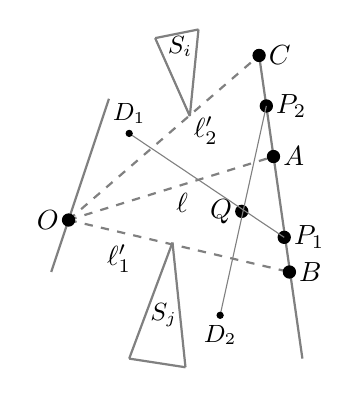
\begin{tikzpicture}[scale = 1.1]
\draw[gray, thick] (0.1, 0) -- (0.7666, 2);
\draw[gray, thick] (3, -1) -- (2.5, 2.5);


\draw[gray, thick] (1, -1) -- (1.5, 0.34);
\draw[gray, thick] (1.65, -1.1) -- (1.5, 0.34);
\draw[gray, thick] (1.65, -1.1) -- (1, -1);

\draw[gray, thick] (1.3, 2.7) -- (1.7, 1.8);
\draw[gray, thick] (1.8, 2.8) -- (1.7, 1.8);
\draw[gray, thick] (1.8, 2.8) -- (1.3, 2.7);

\draw[gray, thick, dashed] (0.3, 0.6) -- (2.66666, 1.333);

\draw[gray, thick, dashed] (0.3, 0.6) -- (2.5, 2.5);
\draw[gray, thick, dashed] (0.3, 0.6) -- (2.85, 0);

\node[text width=1cm] at (2, 0.8) {$\ell$};
\node[text width=1cm] at (2.2, 1.63) {$\ell_2'$};
\node[text width=1cm] at (1.2, 0.15) {$\ell_1'$};

\filldraw[black] (0.3, 0.6) circle (2pt) node[anchor=east] {$O$};
\filldraw[black] (2.666, 1.333) circle (2pt) node[anchor=west] {$A$};
\filldraw[black] (2.5, 2.5) circle (2pt) node[anchor=west] {$C$};
\filldraw[black] (2.85, 0) circle (2pt) node[anchor=west] {$B$};

\filldraw[black] (2.79, 0.4) circle (2pt) node[anchor=west] {$P_1$};
\filldraw[black] (2.5833, 1.917) circle (2pt) node[anchor=west] {$P_2$};

\filldraw[black] (2.3, 0.7) circle (2pt) node[anchor=east] {$Q$};

\draw[gray] (2.79, 0.4) -- (1.0, 1.6);
\draw[gray] (2.5833, 1.917) -- (2.05, -0.5);
\filldraw[black] (1.0, 1.6) circle (1pt) node[anchor=south] {\small{$D_1$}};
\filldraw[black] (2.05, -0.5) circle (1pt) node[anchor=north] {\small $D_2$};


\node[text width=1cm] at (1.9, 2.6) {\small $S_i$};
\node[text width=1cm] at (1.7, -0.5) {\small $S_j$};

\end{tikzpicture}
    \caption{Rotating non-tangent barrier line segment $\ell$ in clockwise and counterclockwise directions around its endpoint $O$ until it becomes tangential to some objects.}
    \label{fig:proof}
    \vspace{-2mm}
\end{figure}
% Then, we show that there exists a set of lines with minimum cardinality that separates $S1$ and $S2$. Similarly, when a line is only tangent to one vertex
\end{proof}

Although we can limit the candidate barriers to line segments tangent to object vertices, there can
still be infinite number of candidates. 
One may consider using line segments that are bitangent to
object vertices, i.e. line segments crossing two object or obstacle vertices. If there are $n$ object/obstacle vertices, there can be at most $n^2$, i.e., a quadratic number of bitangents. 
Unfortunately, bitangent lines are insufficient to act as candidate barriers by themselves for polygonal objects. A counterexample in ~\ref{fig:counter} shows that there is an instance where an optimal solution must contain line segments that are not bitangents. 
%
In this counterexample, we need separate the orange objects from the lime object. A minimum of three line segments are used, and it is not possible that all of them are bitangent, i.e.

\begin{proposition}
Bitangent line segments do not always contain optimal solution for the barrier forming problem for polygonal objects.
\end{proposition}

\begin{figure}[ht]
    \centering
    \vspace{-.2in}
    \includegraphics[width = .25\textwidth]{chapters/bc/fig/counter_example.png}
    \vspace{0.0in}
    \caption{Counterexample that shows using only bitangent line segments cannot create the optimal solution}
    \label{fig:counter}
\end{figure}

Despite the caveat, for the first two formulations that deal with barrier forming for point sets, even with polygonal obstacles, bitangent line segments
always contain an optimal solution. More precisely, 
\begin{theorem}
For any $k$ sets of point objects $S_1, \dots, S_k$ in a workspace $\mathcal W$, there exists
a set of line segments with minimum cardinality that separates $S_1, \dots, S_k$, 
and only consists of bitangent line segments.
\end{theorem}

\begin{proof}
From Theorem~\ref{theorem:sin_tan}, we can see using single tangent line segments is always enough
for an optimal solution. 
Now we turn an optimal solution, $L^*$, with only tangent line segments, into
a solution with only bitangent line segments while still maintaining the same number of barriers. 

For a tangent line segment $\ell=AB\in L^*$ with tangent point $O$ (shown in ~\ref{fig:proof_bi}), and if $O$ is a point object, assume it is beneath $\ell$,
rotate $\ell$ clockwise around $O$ until it hits a point object or an obstacle vertex.
Denote the resulting line segment as $\ell'$, and replace $\ell$ with $\ell'$.
Since the objects are point objects, so $BB'$ and $AA'$ must belong to obstacles or workspace boundary, 
and thus there is no object point inside $OAA'$ or $OBB'$. 
Therefore, the replacement won't result in
any path connecting objects in different classes.
If this is not the case, then there will be some path connecting two object points in different classes that crosses $\ell$ but does not cross $\ell'$ or other barriers. 
Since the triangle areas $OAA'$ and $OBB'$ are empty, that path must enter region $OAA'$ or $OBB'$ and leave them from $\ell$. Then, that part of the path could be replaced with a straight line segment parallel to $\ell$ which prevents it from crossing $\ell$. This contradicts the assumption that $L^*$ prevents all connections between objects in different classes. % of objects.

Continuing the replacement until all line segments are bitangent will result in an optimal solution with only bitangent line segments.

\begin{figure}[ht]
    \centering
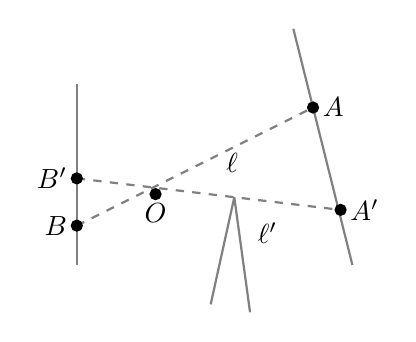
\begin{tikzpicture}
% \draw[gray, thick] (0, 0) -- (1, 2);
\draw[gray, thick] (2.5, -1) -- (1.75, 2);
\draw[gray, thick] (-1, -1) -- (-1, 1.3);

\draw[gray, thick] (0.7, -1.5) -- (1, -0.14);
\draw[gray, thick] (1.2, -1.6) -- (1, -0.14);

% \draw[gray, thick] (3, -1) -- (2.5, 2.5);

% \draw[gray, thick] (1, -1) -- (1.5, 0.34);
% \draw[gray, thick] (1.65, -1.1) -- (1.5, 0.34);
% 
% \draw[gray, thick, dashed] (0.3, 0.6) -- (2.66666, 1.333);
\draw[gray, thick, dashed] (-1., -0.5) -- (2., 1.);

\draw[gray, thick, dashed] (-1., 0.1) -- (2.35, -0.3);

% \draw[gray, thick, dashed] (0.3, 0.6) -- (2.5, 2.5);
% \draw[gray, thick, dashed] (0.3, 0.6) -- (2.85, 0);

\node[text width=1cm] at (1.4, 0.3) 
                        {$\ell$};
% \node[text] at (1.8, 1.63) 
                        % {$\ell_2'$};
\node[text width=1cm] at (1.8, -0.6) 
                        {$\ell'$};

\filldraw[black] (0.0, -0.1) circle (2pt) node[anchor=north] {$O$};
\filldraw[black] (2, 1.) circle (2pt) node[anchor=west] {$A$};
% \filldraw[black] (2.5, 2.5) circle (2pt) node[anchor=west] {$C$};
\filldraw[black] (-1, -0.5) circle (2pt) node[anchor=east] {$B$};

\filldraw[black] (2.35, -0.3) circle (2pt) node[anchor=west] {$A'$};
\filldraw[black] (-1, 0.1) circle (2pt) node[anchor=east] {$B'$};

% \filldraw[black] (2.7583, 0.6666) circle (2pt) node[anchor=west] {$P_1$};
% \filldraw[black] (2.5833, 1.917) circle (2pt) node[anchor=west] {$P_2$};

\end{tikzpicture}
    \caption{Rotating a single tangent barrier line segment $\ell$ around its tangent point $O$ clockwise until it becomes bitangent.}
    \label{fig:proof_bi}
\end{figure}
\end{proof}

For separating polygonal objects, although using bitangent line segments cannot guarantee an optimal solution that uses minimum number of line segments, they can still ensure that solutions limited to bitangents are at least $2$-optimal.
\begin{proposition}
For any $k$ sets of polygonal objects $S_1, \dots, S_k$ in the workspace $\mathcal W$, there exists a set of line segments with cardinality at most twice the minimum cardinality, that separates $S_1, \dots, S_k$, and only consists of line segments that are bitangent to object or obstacle vertices. 
\end{proposition}
\begin{proof}


\begin{figure}[ht]
    \centering
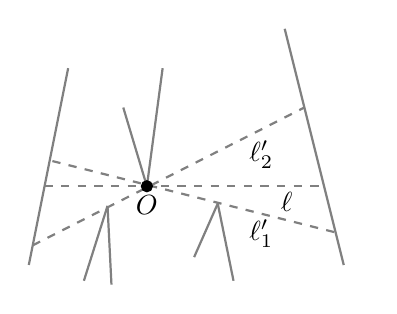
\begin{tikzpicture}

\draw[gray, thick] (2.5, -1) -- (1.75, 2);
\draw[gray, thick] (-1.5, -1) -- (-1, 1.5);
\draw[gray, thick] (0, 0) -- (-0.3, 1);
\draw[gray, thick] (0, 0) -- (.2, 1.5);

\draw[gray, thick] (-0.8, -1.2) -- (-0.5, -0.25);
\draw[gray, thick] (-0.45, -1.25) -- (-0.5, -0.25);

\draw[gray, thick] (0.6, -0.9) -- (0.9, -0.22);
\draw[gray, thick] (1.1, -1.2) -- (0.9, -0.22);


\draw[gray, thick, dashed] (-1.45, -0.75) -- (2., 1.);
\draw[gray, thick, dashed] (-1.3, -0.0) -- (2.2, 0);

\draw[gray, thick, dashed] (-1.2, 0.32) -- (2.45, -0.6);



\node[text width=1cm] at (2.2, -0.2) 
                        {$\ell$};

\node[text width=1cm] at (1.8, -0.6) 
                        {$\ell'_1$};

\node[text width=1cm] at (1.8, 0.4) 
                        {$\ell'_2$};

\filldraw[black] (0.0, -0.0) circle (2pt) node[anchor=north] {$O$};


\end{tikzpicture}
    \caption{Rotating tangent barrier line segment $\ell$ both clockwise and counterclockwise around its tangent point $O$ until it becomes bitangent.}
    \label{fig:proof_bi_2opt}
\end{figure}

Starting from an optimal solution $L^*$ with only tangent line segments,
we will replace each tangent line segment with two bitangent line segments.

Rotate each non-bitangent line segment $\ell\in L^*$ around its tangent point $O$ in clockwise or counterclockwise directions until the line segment become bitangent, as illustrated in ~\ref{fig:proof_bi_2opt}. 
Since any path connecting two objects in different classes and is cut by barrier $\ell$ will still be cut by $\ell'_1$ and $\ell'_2$.
The replacement can still guarantee the separation among the object groups.
After replacing all barriers, we can obtain a 2-OPT solution with the number of line segments twice the minimum.
\end{proof}


\section{Fast Computation of High-Quality Solutions}\label{sec:bf-algorithm}
In this section, we describe three methods for solving infinite-horizon \prob (Problem~\ref{prob:bd-1}).
Sec.~\ref{sec:bd-dp} provide a dynamic programming (DP) algorithm based on one developed in \cite{adler2022role}, 
followed by Sec.~\ref{sec:bd-ilp} formulating an integer linear programming model,
and Sec.~\ref{sec:bd-dp_local} discusses a heuristic search algorithm based on the DP algorithm. 
The extension to an infinite attack stream with a finite look-ahead horizon  (Problem~\ref{prob:bd-2}) will be discussed in Sec.~\ref{sec:bd-hor}.


\subsection{Exact Dynamic Programming Based Method}%for A Fixed Number of Defenders}
\label{sec:bd-dp}

The DP algorithm builds a recursion formula on the last attacks intercepted by the defenders.
Without loss of generality, we assume that each attack is only intercepted by one defender.
For a DP state $a_1, \dots, a_k$ where $a_i$ is the last attack defender $i$ intercepts, 
let $T[a_1]\dots[a_k]$ store the maximum number of attacks that can be intercepted when the $i^{th}$ defender's last intercepted attack events is $a_i$ $(i\in[1,k])$,
and denote $a_{ma}$ as the maximum of $a_1, \dots, a_k$.
Base on which attack the $ma^{th}$ defender intercepts before intercepting attack $a_{ma}$,
we can write the DP recursion formula as follows.
\begin{equation}
\begin{split}
T[a_1]\dots[a_{ma}]\dots[a_k] &= \\ 
\max_{p\in prev(a_{ma}, ma) \wedge p\neq a_1 \dots a_k} &  T[a_1]\dots[p]\dots[a_k] + 1
\end{split}
\end{equation}

Pseudo-code in Alg.~\ref{alg:bd-dp} provides a sketch of a possible implementation of the dynamic programming algorithm.
Effectively implemented, the time complexity of running Alg.~\ref{alg:bd-dp} is $O( (n+1)^{k+1})$, which is polynomial when $k$, the number of defenders, is fixed.
\vspace{-2mm}

\begin{algorithm}
%\begin{small}
\DontPrintSemicolon
\KwData{
$E=\big \langle loc_i, t_i\big\rangle_{i=1}^{n}$: $n$ attack events\;
$loc^1,\dots,loc^k$: initial locations of the $k$ defenders\;
$v_1,\dots,v_k$: speeds of the $k$ defenders\;
}
\KwResult{Maximum number of attacks intercepted}
\vspace{1mm}
$T\gets$ an $(n+1)^k$-length array initialized to $-\infty$\;
\vspace{1mm}
$result\gets 0$\;
\vspace{1mm}
$T[0]\gets 0$\;
\vspace{1mm}
\For{$mask\gets 0 $ \KwTo $(n+1)^k - 1$}{
\vspace{1mm}
    $\overline{a_1 a_2\dots a_k} \leftarrow mask$\;
    \Comment{$\overline{a_1 a_2\dots a_k}$ represents a base-($n+1$) number, i.e., $a_1\cdot (n+1)^{k-1} + a_2 \cdot (n+1)^{k-2} +\dots+ a_k$}
    \If{$\exists\ a_i = a_j$}{
        \Continue\;
    }
\vspace{1mm}
    $ma \leftarrow argmax_i a_i$\;
\vspace{1mm}
    \For{$p\in prev(a_{ma}, ma)$}{
        \If{$\forall i\ pos_i \neq p$}{
            $pm\gets mask - (a_{ma} - p)\cdot (n+1)^{k-ma}$\;
            \Comment{$pm$ is the result of replacing $a_{ma}$ with $p$}
            $T[mask]\gets \max(T[mask], T[pm] + 1)$\;
        }
    }
\vspace{1mm}
    $result\gets \max(result, T[mask])$\;
}
\vspace{1mm}
\Return{$result$}\;

\caption{Dynamic Programming for \prob}
\label{alg:bd-dp}
%\end{small}
\end{algorithm}
\vspace{-2mm}
%\vspace{-15mm}

The algorithm presented here is a slight modification of the DP algorithm in \cite{adler2022role} with two subtle differences. First, we enforce that an attack event can only be handled by one defender.
Second, we explicitly use the initial locations of the defenders in the algorithm, which is essential for handling the finite horizon extension.

\subsection{Solving \prob with Integer Linear Programming Model based on a Flow Formulation}
\label{sec:bd-ilp}

It is not difficult to see that \prob can also be seen as a network flow problem by treating each attack event as a node and the reachability between each pair of attack events for each defender as the edges in the graph. 

Specifically, there are $n$ nodes in the graph, representing the $n$ attack events. 
There are also $O(n^2k)$ connections between nodes inside the graph.
If defender $j$ can reach attack event $i'$ from $i$, there is an connection 
$edge[i][i'][j]$ between node $i$ and $i'$. 
Also, we use a binary variable $intercept[i]$ to denote whether attack event $i$ is successfully intercepted. 
These give rise to the following integer linear programming (ILP) formulation of the problem.

% \begin{gather}
Eq. \eqref{eq:bd-intercept} sets the criteria of an attack $i$ being intercepted as at least one defender to come into the node $i$, which means intercept attack $i$.
Eq. \eqref{eq:bd-flow} sets the defender flow conservation rule that the number of type $j$ defender exiting node $i$ must be larger than or equal to the number of type $j$ defender coming to node $i$.
Eq. \eqref{eq:bd-initial} sets the initial constraints on the number of each type of defender used (coming out from node 0).

\begin{gather}
\sum_{j\in[1, k],\ i'\in prev(i, j)} edge[i'][i][j] \geq intercept[i] \label{eq:bd-intercept}\\
\sum_{nxt_i\in next(i, j)} edge[i][nxt_i][j] \leq \sum_{prv_i \in prev(i,j)} edge[prv_i][i][j]  \label{eq:bd-flow} \\
\sum_{nxt_0 \in next(0, j)} edge[0[nxt_0][j] \leq 1 \label{eq:bd-initial}  \\
Objective\quad \max \sum_i intercept[i]
\end{gather}

% \end{gather}
Denote $M$ as the number of connections in the graph, clearly $M<n^2k$.
This integer linear programming formulation uses $M + n$ variables, and 
$nk + n$ constraints. 

%It may not be worth mentioning
\begin{remark}
The flow formulation of the problem is an NP-hard problem. The proof is similar to the NP-completeness proof of the two-commodity flow in \cite{even1975complexity}. This seems to suggest that \prob is NP-hard as well. 
\end{remark}

% \begin{proof}
% \end{proof}

\subsection{Exhaustive Defenders Pairing Heuristic Search Method}
\label{sec:bd-dp_local}
We now develop a heuristic search method using the dynamic programming algorithm discussed in Alg.~\ref{alg:bd-dp} 
applied on two defenders.
The DP algorithm that computes the optimal solution for two defenders is used as a local improvement primitive 
for the local search heuristic algorithm. 

We call the resulting algorithm \emph{exhaustive defender pairing} (\ours).  
In each iteration, \ours pick two defenders, and the attack events the two defenders have intercepted and the attack events that have not been intercepted by any defender. 
Then, \ours uses the DP algorithm in Alg.~\ref{alg:bd-dp} to increase the number of attack events intercepted by the two defenders selected. 
The complete algorithm is sketched in Alg.~\ref{alg:bd-dp_local}.

\begin{algorithm}[h]
\DontPrintSemicolon
\KwData{
$E=\big \langle loc_i, t_i\big\rangle_{i=1}^{n}$: $n$ attack events\;
$loc^1,\dots,loc^k$: initial locations of the $k$ defenders\;
$v_1,\dots,v_k$: speeds of the $k$ defenders\;
}
\KwResult{Number of attacks intercepted}

$Intercept \gets$ a length-$n$ array initialized to $-1$\;
\Comment{$Intercept$ array stores for each event the defender that intercepts it}
$result\gets 0$\;
\vspace{1mm}
\For{$u, v \in \{1, \dots, k\}\times\{1, \dots, k\}, u\neq v$}{
    $E'\gets \{w\ |\ Intercept[w] \in\{u, v, -1\}\}$ \;
    \Comment{$E'$ stores the set of attack events intercepted by defender $u,v$ and the attacks not intercepted by any defender}
\vspace{1mm}
    $\tilde{n}\gets E'.size$\;
\vspace{1mm}
    T $\gets$ an $(\tilde{n}+1)^2$-length array initialized to $-\infty$\;
\vspace{1mm}
    $T[0]\gets 0$\;
    \Comment{Apply the DP algorithm for defender $u$ and $v$}
\vspace{1mm}
    \For{$mask\gets 0 $ \KwTo $(\tilde{n}+1)^2-1$}{
        $\overline{a_1 a_2} \leftarrow mask$\;
        \If{$a_1 =a_2$}{
            \Continue\;
        }
\vspace{1mm}
        $ma \leftarrow argmax_i a_i$\;
\vspace{1mm}
        \For{$p\in prev(a_{ma}, ma)$}{
            \If{$\forall i\ a_i \neq p$}{
                $pm\gets mask - (a_{ma} - p)\cdot (n+1)^{2-ma}$\;
                $T[mask]\gets \max(T[mask], T[pm] + 1)$\;
            }
        }
        % $result\gets \max(result, T[mask])$\;
    }
\vspace{1mm}
    \If{Solution is improved}{
        Update $Intercept, result$\;
    }
}
\vspace{1mm}
\Return{$result$}
\caption{Exhaustive Defender Pairing}
\label{alg:bd-dp_local}
\end{algorithm}

We can try different defender pairing orders and choose the best one. 
In our \ours implementation, we choose to run line 3 of Alg.~\ref{alg:bd-dp_local} in 3 different iteration ordering of $u, v$.
Alg.~\ref{alg:bd-dp_local}'s running time is $O(k^2 n^3)$ as we try $O(k^2)$ pairs of defenders, and each run of the DP algorithm takes $O(n^3)$.
% ($u$ increasing from $1$ to $k$, decreasing from $k$ to $1$, increasing from $k/2$ to $k$ after which go back to $1$ and increase to $k/2-1$). 

\subsection{Handling Infinite Attack Streams with a Finite Look-Ahead Horizon }
\label{sec:bd-hor}
For Problem~\ref{prob:bd-2} where the attacks $\big \langle loc_i, t_i\big \rangle_{i=1}^{\infty}$ may be infinite, and the look-ahead horizon is finite, not all attacks are revealed at once. As such, previous methods cannot be directly applied. 
As the future attack sequence cannot be foreseen, defenders need to \emph{react} to information (e.g., the attack events in the next $T$ time interval) obtained so far. 

Towards addressing the problem, a greedy \emph{replanning} approach can be applied. Whenever an attack event is observed, the defender team replans the capture sequence given the new attacks added to the attack queue. 
This gives rise to an online algorithm sketched in Alg.~\ref{alg:bd-horizon}.

\begin{algorithm}[h]
\DontPrintSemicolon
\KwData{
$E=\big \langle loc_i, t_i\big\rangle_{i=1}^{\infty}$: a stream of attack events\;
$loc^1,\dots,loc^k$: initial locations of the $k$ defenders\;
$v_1,\dots,v_k$: speeds of the $k$ defenders\;
}
$E'\gets $ an empty queue\;
\Comment{$E'$ stores attack events seen so far}
\vspace{1mm}
\While{new attack events added to $E'$ }{
    Apply Alg.~\ref{alg:bd-dp_local} to compute a plan for the defenders and attack events $E'$\;
    Execute the plan, pop out from $E'$ attack events passed, and update $loc^1,\dots,loc^k$ to the defenders' current locations until new attacks are foreseen\;
}
% \KwResult{Number of attacks intercepted}

% $Intercept \gets$ a length-$n$ array initialized to $-1$\;
% \Comment{$Intercept$ array stores for each event the defender that intercepts it}
% $result\gets 0$\;
% \For{$u, v \in \{1, \dots, k\}\times\{1, \dots, k\}, u\neq v$}{
%     $E'\gets \{w\ |\ Intercept[w] \in\{u, v, -1\}\}$ \;
%     \Comment{$E'$ stores the set of attack events intercepted by defender $u,v$ and the attacks not intercepted by any defender}
%     $\tilde{n}\gets E'.size$\;
%     T $\gets$ an $(\tilde{n}+1)^2$-length array initialized to $-\infty$\;
%     $T[0]\gets 0$\;
%     \For{$mask\gets 0 $ \KwTo $(\tilde{n}+1)^2-1$}{
%         $\overline{a_1 a_2} \leftarrow mask$\;
%         \If{$pos_0 = pos_1$}{
%             \Continue\;
%         }
%         $ma \leftarrow argmax_i pos_i$\;
%         \For{$p\in prev(a_{ma}, ma)$}{
%             \If{$\forall i\ pos_i \neq p$}{
%                 $T[mask]\gets \max(T[mask], 1 + T[\overline{a_1\dots p \dots a_k}])$\;
%             }
%         }
%         % $result\gets \max(result, T[mask])$\;
%     }
%     \If{Solution is improved}{
%         Update $Intercept, result$\;
%     }
% }
% \Return{$result$}
\caption{Online Exhaustive Defender Pairing}
\label{alg:bd-horizon}
\end{algorithm}

\section{Experimental Evaluation}\label{sec:bf-evaluation}
In this section, we describe our experimental study of the method proposed in the paper.
Four settings were used to account for the three variants of the barrier forming, the instances and solution examples of which are shown in ~\ref{fig:bf-exp}. 
The experiments were carried out on a Hexa-Core processor with 16 GiB memory, and Gurobi
\cite{optimization2019gurobi} was used as the Integer Programming solver.
In the polygonal object instances generation, random polygons were generated by computing traveling salesperson tour (TSP) tours of random point sets each consisting of $3$ to $6$ vertices, which we found to be effective in generating sensible looking polygons that are not necessarily convex.
%
When a problem setup contains obstacles, the number of obstacles in the environment is set to be the same as the number of objects for each object set.


\begin{figure*}[ht]
    \centering
    
    \includegraphics[trim=80 20 80 20,clip, width = .24\textwidth]{chapters/bf/fig/exp_1_instance.png}
    \hspace{-.1in}
    \includegraphics[trim=80 20 80 20,clip, width = .24\textwidth]{chapters/bf/fig/exp_1_result.png}
    \includegraphics[trim=80 20 80 20,clip, width = .24\textwidth]{chapters/bf/fig/exp_2_instance.png}
    \hspace{-.1in}
    \includegraphics[trim=80 20 80 20,clip, width = .24\textwidth]{chapters/bf/fig/exp_2_result.png}
    \includegraphics[trim=80 20 80 20,clip, width = .24\textwidth]{chapters/bf/fig/exp_3_instance.png}
    \hspace{-.1in}
    \includegraphics[trim=80 20 80 20,clip, width = .24\textwidth]{chapters/bf/fig/exp_3_result.png}
    \includegraphics[trim=80 20 80 20,clip, width = .24\textwidth]{chapters/bf/fig/exp_4_instance.png}
    \hspace{-.1in}
    % \includegraphics[trim=80 20 80 20,clip, width = .24\textwidth]{fig/exp_4_result.png}
    \begin{overpic}[trim=80 20 80 20,clip, width = .24\textwidth]{chapters/bf/fig/exp_4_result.png}
    \put(-202, 98) {(a)}
    \put(-3, 98) {(b)}
    \put(-202, 0) {(c)}
    \put(-3, 0) {(d)}
    
    \end{overpic}
    \caption[Illustration of the four types of instances used in our  experimental evaluation]{Illustration of the four types of instances used in our  experimental evaluation. (a) Barrier forming for point sets. (b) Barrier forming to separate point sets from polygonal obstacles. (c) Barrier forming to separate uniform square-shaped objects among uniform square-shaped obstacles. (d) Barrier forming to separate random polygonal objects among random polygonal obstacles.}
    \label{fig:bf-exp}
\end{figure*}

\subsection{Separating Sets of Points}
The first type of instances aims at forming barriers among randomly generated point sets, 
shown in ~\ref{fig:bf-exp}(a). The number of object sets to separate from each other range from $2$ to $4$, 
and the number of objects in each set range from $1$ to $6$. 
Each entry in the ~\ref{tab:bf-expr_1} is the result of average computation times over 10 instances. From the result, we observe that the IP based method is fairly effective in separating two sets of objects with the presence of obstacles. The method scales to about $10$ point objects plus obstacles. The number of line segments in the optimal barrier are generally small, e.g., $3$-$10$.

\begin{table}[ht]
    \centering
    \begin{tabular}{|c|c|c|c|c|c|c|}\hline
        %  \diagbox{\#Set}{\#Objects}
        \#Sets &  1 & 2 & 3 & 4& 5& 6\\\hline
    2& 0.005 & 0.011 & 0.083 & 0.419 & 2.010 & 15.887 \\\hline
    3& 0.013 & 0.316 & 12.773 & 962.883 & - & - \\\hline
    4& 0.051 & 14.641 &  -& - &  -&- \\\hline
    \end{tabular}
    \caption[Running time in seconds for Expr. 1]{Running time in seconds for Expr. 1 where all objects and obstacles are points (~\ref{fig:bf-exp}(a)). ``-'' denotes the result cannot be computed in 1h on average (the same is true for other tables). 
    The column index means the number of objects in each set, and the row index means the number of object sets.
    The number of obstacles is set to be the same as the number of objects for each set. These also apply to the following tables.
    }
    \label{tab:bf-expr_1}
\end{table}

 The second type of instances generates barriers for randomly generated 
 point sets with the existence of polygonal obstacles, shown in ~\ref{fig:bf-exp}(b). 
 The other specification is the same as Expr. 1, and the number of obstacles for each experiment is set to be the same as the number of objects for each set. 
 The resulting time cost, shown in \ref{tab:bf-expr_2}, is similar to Expr. 1 despite the existence of obstacles.
 %
 Similarly, we observe decent performance when it comes to separating two sets of objects among obstacles. 
 %
 The introduction of polygonal obstacles does not cause performance degradation. 


\begin{table}[ht]
    \centering
    \begin{tabular}{|c|c|c|c|c|c|c|}\hline
        %  \diagbox{\#Set}{\#Objects}
        \#Set &  1 & 2 & 3 & 4& 5& 6\\\hline
2& 0.009 & 0.061 & 0.480 & 5.899 & 3.433 & 21.121\\\hline
 3& 0.044 & 3.287 & 71.346 & 320.955 & - & -\\\hline
 4& 0.249 & 13.801 & - & - & - & -\\\hline
    \end{tabular}
    \caption[Running time in seconds for Expr. 2]{Running time in seconds for Expr. 2 where objects to be separated are points and obstacles are randomly generated polygons (~\ref{fig:bf-exp}(b)). 
    }
    \label{tab:bf-expr_2}
    \vspace{-2mm}
\end{table}
 
\subsection{Separating Sets of Polygonal Shapes}
The third set of experiments uses randomly placed squares as obstacles and objects, shown in ~\ref{fig:bf-exp}(c). The squares are sampled from a $7\times7$ grid. Each square is half the scale of a grid cell and is positioned at the center of a grid cell. The running time for this case turns out to be the greatest among all $4$ experiments. This is due to the rectlinear nature of the instance, which creates many small cells that are difficult to process. 

\begin{table}[ht]
    \centering
    \begin{tabular}{|c|c|c|c|c|c|c|}\hline
        %  \diagbox{\#Set}{\#Objects}
         \#Set &  1 & 2 & 3 & 4& 5& 6\\\hline
 2 & 0.010 & 0.065 & 0.652 & 31.536 & 575.933 & 1259.653\\\hline
 3 & 0.065 & 10.608 & 337.050 & - & - & -\\\hline
 4 & 0.235 & 124.963 & - & - & - & -\\\hline
    \end{tabular}
    \caption[Running time in seconds for Expr. 3]{Running time in seconds for Expr. 3 with square-shaped objects and obstacles (~\ref{fig:bf-exp}(c)). ``-'' denotes the result cannot be computed in 1h on average. 
    % The number of obstacles is set to be the same as the number of objects for each set.
    }
    \label{tab:bf-expr_3}
    \vspace{-2mm}
\end{table}
 
The last type of instances uses random polygons with $3\sim 6$ vertices
as objects and obstacles, shown in ~\ref{fig:bf-exp}(d). 
Counter intuitively, these experiments turn out to have the least time cost among the $4$ experiments despite the most complex environment; we see that even for four different sets of objects where each set contains six objects, the problem can be solved very quickly. %This is due to the larger area of the object sets, which limits the choices of barrier line segments. 

In the end, the running time of the algorithm provided is more dependent on the number of cells and candidate barrier line segments. 
When objects and obstacles are more densely packed in the experiment, 
there will be less barrier candidates and cells due to collisions between objects and the candidate line segments.
While in a sparse environment or even with just point objects, there will be more barrier candidates and cells.
This explains the reduced time cost in a more complex environment from the sparse settings.

\begin{table}[ht]
    \centering
    \begin{tabular}{|c|c|c|c|c|c|c|}\hline
        %  \diagbox{\#Set}{\#Objects}
         \#Set&  1 & 2 & 3 & 4& 5& 6\\\hline
2& 0.006 & 0.031 & 0.080 & 0.143 & 0.157 & 0.156 \\\hline
3& 0.031 & 0.234 & 0.994 & 1.271 & 1.980 & 1.187 \\\hline
4& 0.103 & 0.518 & 3.000 & 6.050 & 9.692 & 17.996 \\\hline 
    \end{tabular}
    \caption[Running time in seconds for Expr. 4]{Running time in seconds for Expr. 4 where both the objects to be separated and the obstacles are randomly generated polygons 
    (~\ref{fig:bf-exp}(d)).
    % The number of obstacles is set to be the same as the number of objects for each set.
    }
    \label{tab:bf-expr_4}
    \vspace{-2mm}
\end{table}
